\documentclass[12pt, titlepage]{article}


\usepackage{pifont}
\usepackage{booktabs}
\usepackage{tabularx}
\usepackage{pdfpages}
\usepackage{graphicx}
\usepackage{hyperref}
\usepackage{enumitem}
\usepackage{changepage}
\usepackage{tabto}
\usepackage{mdframed}
\usepackage{xkeyval}
\usepackage[round]{natbib}
\usepackage{soul}
\usepackage{color}

\hypersetup{
    colorlinks,
    citecolor=black,
    filecolor=black,
    linkcolor=red,
    urlcolor=blue
}
%% the following adds another section level by redefining the paragraph
%% source:  http://tex.stackexchange.com/questions/60209/how-to-add-an-extra-level-of-sections-with-headings-below-subsubsection
\setcounter{secnumdepth}{4}




%% Comments
\newif\ifcomments\commentstrue

\ifcomments
\newcommand{\authornote}[3]{\textcolor{#1}{[#3 ---#2]}}
\newcommand{\todo}[1]{\textcolor{red}{[TODO: #1]}}
\else
\newcommand{\authornote}[3]{}
\newcommand{\todo}[1]{}
\fi

\newcommand{\wss}[1]{\authornote{magenta}{SS}{#1}}
\newcommand{\ds}[1]{\authornote{blue}{DS}{#1}}



%% The following are used for pretty printing of events and requirements
\makeatletter

\define@cmdkey      [TP] {test}     {name}       {}
\define@cmdkey      [TP] {test}     {desc}       {}
\define@cmdkey      [TP] {test}     {type}       {}
\define@cmdkey      [TP] {test}     {init}       {}
\define@cmdkey      [TP] {test}     {input}      {}
\define@cmdkey      [TP] {test}     {output}     {}
\define@cmdkey      [TP] {test}     {pass}       {}
\define@cmdkey      [TP] {test}     {user}       {}


\newcommand{\getCurrentSectionNumber}{%
  \ifnum\c@section=0 %
  \thechapter
  \else
  \ifnum\c@subsection=0 %
  \thesection
  \else
  \ifnum\c@subsubsection=0 %
  \thesubsection
  \else
  \thesubsubsection
  \fi
  \fi
  \fi
}

\newcounter{TestNum}

\@addtoreset{TestNum}{section}
\@addtoreset{TestNum}{subsection}
\@addtoreset{TestNum}{subsubsection}

\newcommand{\testauto}[1]{
\setkeys[TP]{test}{#1}
\refstepcounter{TestNum}
\begin{mdframed}[linewidth=1pt]
\begin{tabularx}{\textwidth}{@{}p{3cm}X@{}}
{\bf Test \getCurrentSectionNumber.\theTestNum:} & {\bf \cmdTP@test@name}\\[\baselineskip]
{\bf Type:} & \cmdTP@test@type\\[0.5\baselineskip]
{\bf Initial State:} & \cmdTP@test@init\\[0.5\baselineskip]
{\bf Input:} & \cmdTP@test@input\\[0.5\baselineskip]
{\bf Output:} & \cmdTP@test@output\\[0.5\baselineskip]
{\bf Pass:} & \cmdTP@test@pass
\end{tabularx}
\end{mdframed}
}

\newcommand{\testautob}[1]{
\setkeys[TP]{test}{#1}
\refstepcounter{TestNum}
\begin{mdframed}[linewidth=1pt]
\begin{tabularx}{\textwidth}{@{}p{3cm}X@{}}
{\bf Test \getCurrentSectionNumber.\theTestNum:} & {\bf \cmdTP@test@name}\\[\baselineskip]
{\bf Description:} & \cmdTP@test@desc\\[0.5\baselineskip]
{\bf Type:} & \cmdTP@test@type\\[0.5\baselineskip]
{\bf Pass:} & \cmdTP@test@pass
\end{tabularx}
\end{mdframed}
}

\newcommand{\testmanual}[1]{
\setkeys[TP]{test}{#1}
\refstepcounter{TestNum}
\begin{mdframed}[linewidth=1pt]
\begin{tabularx}{\textwidth}{@{}p{3cm}X@{}}
{\bf Test \getCurrentSectionNumber.\theTestNum:} & {\bf \cmdTP@test@name}\\[\baselineskip]
{\bf Description:} & \cmdTP@test@desc\\[0.5\baselineskip]
{\bf Type:} & \cmdTP@test@type\\[0.5\baselineskip]
{\bf Tester(s):} & \cmdTP@test@user\\[0.5\baselineskip]
{\bf Pass:} & \cmdTP@test@pass
\end{tabularx}
\end{mdframed}
}


\makeatother

\newcommand{\ZtoT}{
\begin{tabularx}{3.85cm}{@{}p{0.35cm}p{0.35cm}p{0.35cm}p{0.35cm}p{0.35cm}p{0.35cm}@{}}
0 & 1 & 2 & 3 & 4 & 5 
\end{tabularx}}

\title{\parbox{\linewidth}{\centering Test Plan\endgraf\bigskip Super Tetris}}
\author{\parbox{\linewidth}{\bigskip \centering Group\#: 38 \endgraf\bigskip Team Name: Binary \endgraf\bigskip Members: \endgraf\bigskip Tongfei Wang : wangt62 \endgraf\bigskip Bowen Yuan : yuanb1 \endgraf\bigskip Tim Zhang : zhangj14}}
\date{\parbox{\linewidth}{\bigskip\bigskip \centering \today\endgraf\bigskip SFWR ENG 3XA3 \endgraf\bigskip McMaster University}}


\begin{document}
\maketitle

\pagenumbering{roman}
\tableofcontents
\listoftables
\listoffigures

\begin{table}[bp]
\caption{\bf Revision History}
\begin{tabularx}{\textwidth}{p{3cm}p{2cm}X}
\toprule {\bf Date} & {\bf Version} & {\bf Notes}\\
\midrule
Oct 27 2017 & 1.0 & General Info \& Plan Uploaded\\
Oct 27 2017 & 1.1 &  System Test Descriiption Uploaded\\
Oct 27 2017 & 1.2 & Tests for PoC Uploaded\\
Oct 27 2017 & 1.3 & Unit Testing Plan Uploaded\\
\bottomrule
\end{tabularx}
\end{table}

\newpage

\pagenumbering{arabic}

\section{General Information}

\subsection{Purpose}
\tab The purpose is to test Super Tetris which is re-implemented from the Tetris game. This document will make a test plan which shall have a testing structure. Following the structure, several test cases shall be able to generate . \st{and test both functional and non-functional requirements.} {\color{red} The test cases cover both funcitonal and non-functional requirements.}

\subsection{Scope}
 \tab As the purpose is to test a software project, the tests shall meet both functional and non-functional requirements.\\
 For functional requirement, \st{is} {\color{red} it} shall test all classes and functions of the program including the original codes. In term of non-functional requirement, it shall test if the program meets the developing requirement and \st{all} if all the added elements works well. Also, the added icons, pictures, and \st{anime} {\color{red} animation} shall appear at the right place \st{at} {\color{red} and} a right time.

\subsection{Acronyms, Abbreviations, and Symbols}
	
\begin{table}[hbp]
\caption{\textbf{Table of Abbreviations}} \label{Table}

\begin{tabularx}{\textwidth}{p{3cm}X}
\toprule
\textbf{Abbreviation} & \textbf{Definition} \\
\midrule
POC & Proof of Concept\\
FR & Functional Requirement\\
NFR & Non-Functional Requirement\\
NFR & Non-Functional Requirement\\
SP & Super Tetris\\
IN & Input and Navigation\\
GL & Game Logic\\
\bottomrule
\end{tabularx}

\end{table}

\begin{table}[!htbp]
\caption{\textbf{Table of Definitions}} \label{Table}

\begin{tabularx}{\textwidth}{p{3cm}X}
\toprule
\textbf{Term} & \textbf{Definition}\\
\midrule
Tetrominoes & Geometric shape composed of four squares\\
Item &  Four different items to help player get higher scores\\
Line Clear & Theway to obtain score in Super Tetris\\
Score & Measure of Player's performance\\
\bottomrule
\end{tabularx}
\end{table}	

~\newline
\subsection{Overview of Document}
\tab  \st{In this document, it will make a plan for the testing.} {\color{red} This document shows the testing plan in detail.}At first, the document will briefly introduce the software to be tested, test team and the testing tools. Secondly, according to the scope of testing, it will talk about the details about the implemented function to be tested and the way it works. The article will also clarify that how the test team overcomes the challenging testing. As the unit testing \st{shall be used} {\color{red} is used  and } it is essential  {\color{red} part of our testing process } \st{to introduce the plan to it at last}{\color{red} ,the introduction  of it will be at the end of this document}  .

\section{Plan}
	
\subsection{Software Description}
\tab Tetris is a tile-matching puzzle game. "Tetrominoes" are differently shaped blocks and they drop from the top of the screen one by one. The player can move or rotate the Tetriminos as they fall. The goal of this game is to create a horizontal line without gaps {\color{red} to gain the score of the game.}
\st{Once the line is created, it will disappear and be replaced by the blocks above it.}

\subsection{Test Team}
\tab The test team will consist of Tim Zhang, Bowen Yuan, Tongfei Wang. The three main testers will split the entire testing evenly covering all the different types of testing and preparing the automated testing.

\subsection{Automated Testing Approach}
\tab Automated testing will be used for testing of the game mechanics system and {\color{red} it} will utilize both unit testing and coverage analysis. To ensure that unit testing can be run while the game mechanics are in development the test cases have been grouped into sections that can be fully implemented once certain subsets of the game mechanics systems are completed.

\subsection{Testing Tools}
\tab Super Tetris is programmed in Javascript, So we decide to use 'Mocha' to automate the unit testing.

\subsection{Testing Schedule}

\begin{table}[!htbp]
\centering
	\begin{tabular}[pos]{|l|c|r|}
		\hline
		\color{red}\textbf{Task}& \color{red}\textbf{Team Member} & \color{red}\textbf{Date} \\ \hline
		User Input&Bowen&Oct 30th 2017\\ \hline
		Navigation&Bowen&Nov 4th 2017 \\ \hline
		Game Logic&Micho&Nov 4th 2017 \\ \hline
		Usability&Tim &Nov 10th 2017 \\ \hline
		Performance&Micho&Nov 10th 2017 \\ \hline
		
	\end{tabular}
		\caption{Testing Assignments}
		\label{Table}	
	
\end{table}	

		
See Gantt Chart at the following url ...

\section{System Test Description}


%%%%%%%%%%%%%%%%%%%%%%%
\subsection{Tests for Functional Requirements}

\subsubsection{User Input and Navigation Test }


\testauto{
    name = {SP-IN1},
    type = {Functional,Dynamic,Manual},
    init =Web browser is open,
    input =  User enters the domain of this game,
    output = A new game starts,
    pass = We will use different \st{mobile devices and PC} {\color{red}browsers} to check if the game interface is displayed successfully after entering our game domain \st{in web browser}.
}

\testauto{
    name = {SP-IN2},
    type = {Functional,Dynamic,Manual},
    init =Game is in process,
    input =  User presses 'enter',
    output = Game paused,
    pass = We will check if game is paused after pressing 'enter' when game is in process.
}


\testauto{
    name = {SP-IN3},
    type = {Functional,Dynamic,Manual},
    init =Game is paused,
    input =  User presses 'enter',
    output = Game resumes,
    pass = We will check if game is resumed successfuly after pressing 'enter' when game is paused
}
					

\testauto{
    name = {SP-IN4},
    type = {Functional,Dynamic,Manual},
    init = Game is paused or in process,
    input =  User presses 'r',
    output = Game is restarted ,
    pass = We will check if game is restarted successfuly after pressing 'r' when game is paused or in process
}


\testauto{
name = {SP-IN5},
type = {Functional,Dynamic,Manual},
init = Game is in process,
input =  User presses \st{'up'}  {\color{red} 'w'},
output =  The current tetromino is rotated clockwise,
pass = We will check if the current tetromino is rotated clockwise when user presses 'up'
}

\testauto{
name = {SP-IN6},
type = {Functional,Dynamic,Manual},
init = Game is in process,
input =  User presses 'left' or 'right' by one grid,
output =  The current tetromino is moved left/right ,
pass = We will check if the current tetromino is moved left/right by exactly one gird when user presses 'left' or 'right'.
}

\testauto{
name = {SP-IN7},
type = {Functional,Dynamic,Manual},
init = Game is in process,
input =  User presses 'down’,
output =  The current tetromino falls to the bottom(not intersected with other tetrominoes)  ,
pass = We will check if the current tetromino falls to the bottom when user presses 'down'
}

\testauto{
name = {SP-IN8},
type = {Functional,Dynamic,Manual},
init = Game is in process,
input =  User presses '1' or '2' or '3' \st{or ‘4’},
output =  User buys and uses the item they selected('1' to \st{'4'} {\color{red} '3'} correspanding to four different items), 
pass = We will check if users can use the item they selected successfully when they press '1' to \st{'4'} {\color{red} '3'}
}



%%%%%%%%%%%%%%%%%%%%%%%%%%
\subsubsection{Game Logic Test}
~\newline

\testauto{
name = {\st{SP-GL1}},
type = {\st{Structrual,Dynamic,Automated}},
init = \st{Game is in Process.},
input =  \st{a 4*4 (represent a certain tetromino)},
output = \st{a 4*4matrix(represent an input tetromino rotating 90 degrees clockwise)},
pass =  \st{We will use assert to check if function rotateRight matrix) can accept a 4*4 metrix and return a 4*4   matrix rotating 90 degrees clockwise. }
}


\testauto{
name = {SP-GL2},
type = {Structrual,Dynamic,Automated},
init = Game is in Process.,
input =  Coordinate of current tetromino which is a 4*4 \st{metrix} {\color{red} matrix},
output =  Boolean,
pass =  We will use assert to check if function intersects can judge the current tetromino intersects the border or other tetrominoes. 
}

\testauto{
name = {SP-GL3},
type = {Structrual,Dynamic,Automated},
init = Game is in Process.,
input =  row number,
output =  new row or number of rows killed,
pass =  We will use assert to check if funcion killrows() can kill a(some) filled row and increase the number of rows killed
}

\testauto{
name = {SP-GL4},
type = {Structrual,Dynamic,Automated},
init = Game is in Process.,
input =  N/A,
output =  A random 4*4 piece(tetromino),
pass = We will use assert to check if function randomPiece() can return a 4*4 \st{metrix} {\color{red} matrix} (any tetromino) randomly.
}

\testauto{
name = {\st{SP-GL5}},
type = {\st{Structrual,Dynamic,Automated}},
init = \st{Game is in Process.},
input =  \st{N/A},
output =  \st{A playfield can be drawed} ,
pass =  \st{We will use assert to check if function newGame() can create a 20*10 playfield successfully}.
}

\testauto{
name = {\st{SP-GL6}},
type = {\st{Structrual,Dynamic,Automated}},
init = \st{Game is in Process.},
input =  \st{Number of rows killed} ,
output =  \st{Experience},
pass = \st{ We will use assert to check if function getExp() can return the number of Experience which Experience = 10*number of rows killed }
}

\testauto{
name = {SP-GL7},
type = {Structrual,Dynamic,Automated},
init = Game is in Process.,
input =  item,
output =  boolean,
pass =  We will use assert to check if function haveEnoughMoney() can return whether a user can buy the item he selected 
}

\testauto{
name = {\st{SP-GL8}},
type = {\st{Structrual,Dynamic,Automated}},
init = \st{Game is in Process.},
input =  \st{price of item} ,
output =  \st{Experience},
pass = \st{ We will use assert to check if function newExp() can return whether the remaining Exp when user bought certain item.}
}

\testauto{
name = {SP-GL9},
type = {Structrual,Dynamic,Automated},
init = Game is in Process.,
input =  Number of rows killed£¨playing time,
output =  Score,
pass =  We will use assert to check if function getScore() can return the number of Score which Score \= 100*number of rows killed + 10*time(second)
}

\testauto{
name = {SP-GL10},
type = {Structrual,Dynamic,Automated},
init = Game is in Process.,
input =  N/A,
output =  speed of falling,
pass =  We will use assert to check if function useSlow() can return the speed of falling which is half of original speed and lasts 30 seconds.
}

\testauto{
name = {SP-GL11},
type = {Structrual,Dynamic,Automated},
init = Game is in Process.,
input =  N/A,
output =  4*4 \st{metrix} {\color{red} matrix}  ,
pass =  We will use assert to check if function useSkip() can return a new random 4*4 \st{metrix} {\color{red} matrix} which override the original \st{metrix} {\color{red} matrix}.
}

\testauto{
name = {SP-GL12},
type = {Structrual,Dynamic,Automated},
init = Game is in Process.,
input =  N/A,
output =  rows or number of row killed,
pass =  We will use assert to check if function useClear() can kill the top row and return the new rows and \st{increse} {\color{red} increase} the number of row{\color{red}s} killed.
}

\testauto{
name = {SP-GL13},
type = {Structrual,Dynamic,Automated},
init = Game is in Process.,
input =  Playfield,
output =  Boolean,
pass =  We will use assert to check if function gameover() can return the game is over or not.(When part of a new tetromino(or the whole part) cannot be displayed in game playfield because of collision with other tetrominoes that game is over)
}

\testauto{
name = {SP-GL14},
type = {Structrual,Dynamic,Automated},
init =State: Game is paused,
input =  N/A,
output =  Exception,
pass =  When user tries to move the tetromino when game is paused then a exception will be raised.
}
%%%%%%%%%%%%%%%%%%%%%%%%%%

\subsection{Tests for Nonfunctional Requirements}

\subsubsection{Performance}

\testmanual{
    name = Precision,
    desc =The event shall happen at the correct time. ,
    type = {Functional (dynamic, manual)},
    user = Development team,
    pass = {The boom shall explode when it stops. The ice shall slow the falling time when it is triggered. The line shall be cleared when a complete line is made.}
}
	
\testmanual{
    name = Capacity,
    desc = Super Tetris needs less than 10MB in memory. ,
    type = {Functional (dynamic, manual)},
    user = Development team,
    pass = {Test team calculates the size of whole program file before uploading.}
}				




%%%%%%%%%%%%%%%%%%%%%%%%%%%%%%%%%%%
\subsubsection{Usability}

\testmanual{
    name = Operating System Support,
    desc = Super Tetris shall run on all major web browsers ( Chrome/Firefox/Safari /IE) ,
    type = {Functional (dynamic, manual)},
    user = Development team,
    pass = {Test team run and play the game through Chrome/Firefox/Safari /IE.}
}				

\testmanual{
    name = Look and Feel,
    desc = The falling of the tetrimino and line clear requires animation,
    type = {Functional (dynamic, manual)},
    user = Development team,
    pass = {When tetriminos are falling or when a row is eliminated, the animation display correctly.}
}		

\testmanual{
    name = Difficulty,
    desc = Super Tetris shall follow the same rule in the Classic Tetris. ,
    type = {Functional (dynamic, manual)},
    user = Development team,
    pass = {Average survey score of less than 4 in 'Difficulty' section.}
}		




%%%%%%%%%%%%%%%%%%%%%%%%%%%%%%%%%%%%%
\subsection{Traceability Between Test Cases and Requirements}
\tab  All the failure test cases shall throw exception which shows where the issue from.
\begin{figure}
\centering
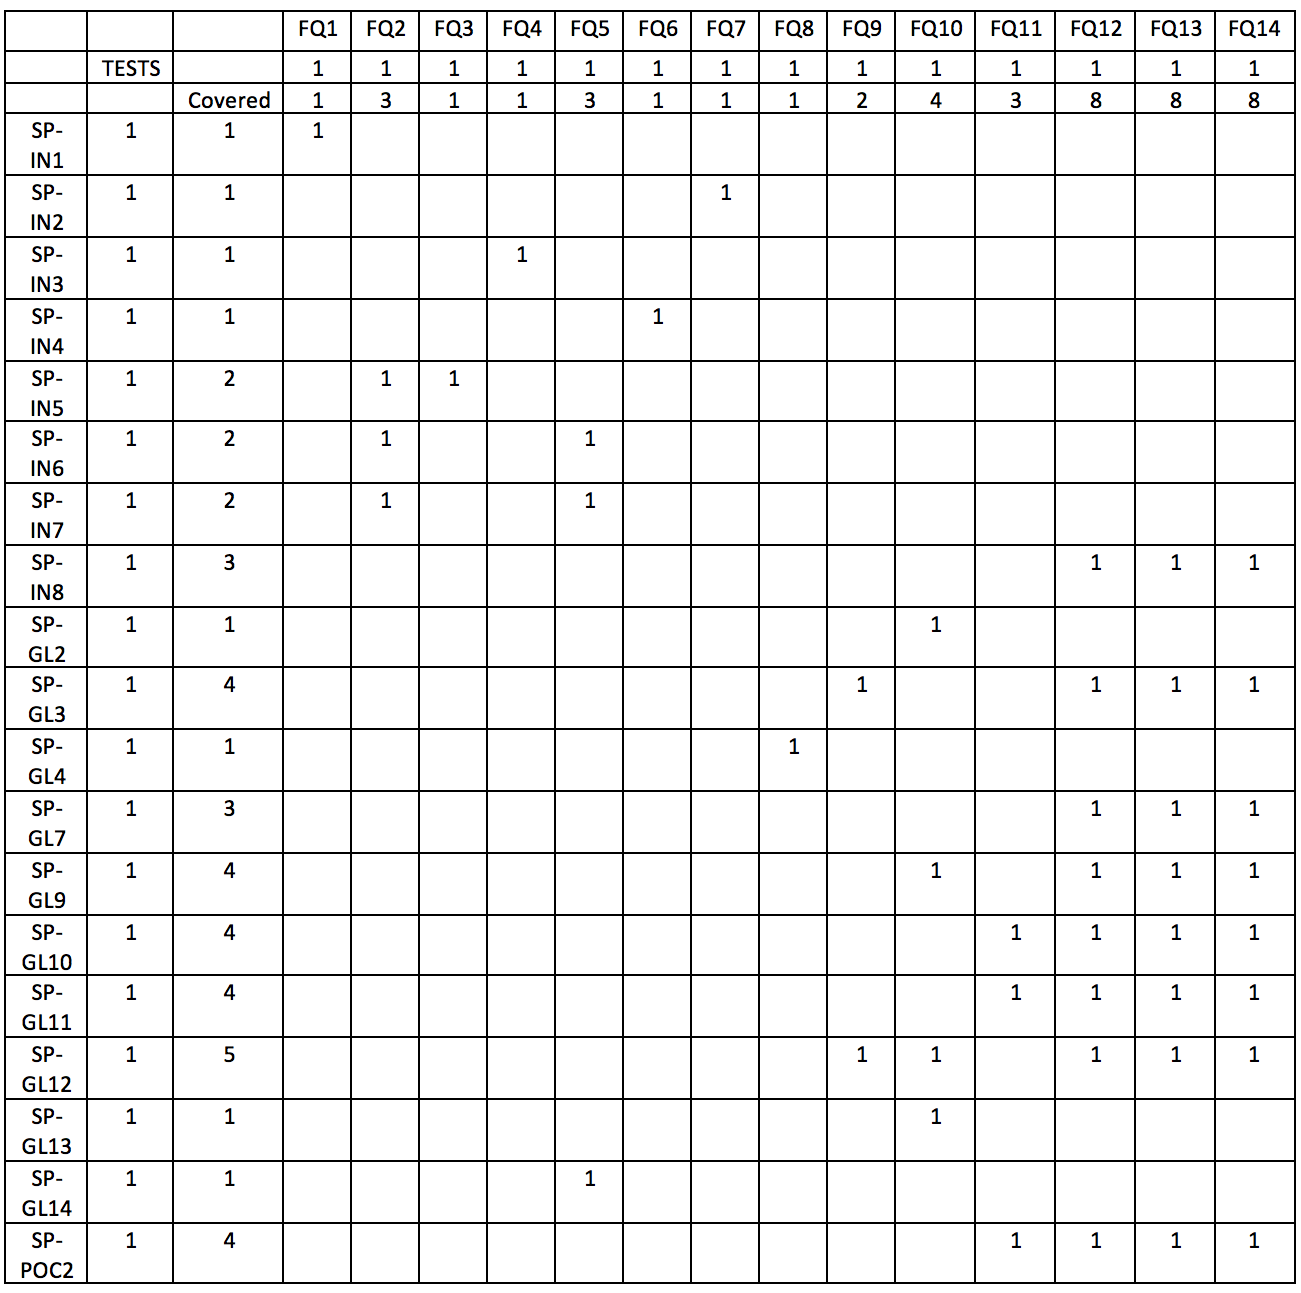
\includegraphics[width=0.9\textwidth]{trace.png}
\caption{{\color{red}Traceability Testing Matrix}}
\label{FigUH}
\end{figure}


\section{Tests for Proof of Concept}
\st{REDRAW TEST}
\testauto{
name = {\st{SP-POC1}},
type = {\st{Dynamic,Manual}},
init = \st{Game over},
input =  \st{User presses 'r' or refresh  the browser} ,
output =   \st{New playfield replaces the original playfield and empty the score and Exp}.  ,
pass = \st{Press 'r' or refresh the website}
}

BOMB TEST
\testauto{
name = {SP-POC2},
type = {Dynamic,Manual},
init =  Game is in process,
input =  user presses '1' ,
output = Bomb is used ,
pass = Press '1' and use a bomb to test to check if the 5*5 area around the bomb has been cleared up. 
}

{\color{red}The tests of Proof of Concept, we will use test SP-IN8, SP-GL7, SP-GL9, SP-GL10 as we describe above}

	
\section{Comparison to Existing Implementation}	
\tab  There shall be a separate package called testing in the program. The package shall include several classes with different testing methods. The classed shall invoke the methods and functions implemented without changing them. That is to say, all the implementation shall not be affected and remain unchanged after the testing.
\section{Unit Testing Plan}
 ‘Mocha’ shall be used as tool for unit testing. 


\subsection{Unit testing of internal functions}
\tab  In order to test the internal functions,  a unit test will be used to test most of the classes and methods implemented. We will generate a sequence of moves as input values. The sequence shall cover most implemented functions. The unit test shall use calculate right output values by math or logic. After that, it shall check whether the outputs match the right ones. It will throw exceptions if the program outputs a wrong value. Finally, a test coverage metrics will be used so as to calculate the how much percentage does the unit test include. At least 75 percent of the functions should be included.

\subsection{Unit testing of output files}		
\tab  As the testing going, the interface of the game will change accordingly. The test will set several testing points in order to check if the  \st{anime} {\color{red} animation}  and graphs go well. It shall take one screenshot of the interface per point. Also, as the test going, it shall generate the graphs according to the methods used as right outputs. Then, the similarity of both outputs shall be checked. At least a similarity of 98 percent shall be considered acceptable. For the cases below 98 percent, it will throw exceptions.

\bibliographystyle{plainnat}

\bibliography{SRS}

\newpage

\section{Appendix}

This is where you can place additional information.

\subsection{Symbolic Parameters}


\subsection{Usability Survey Questions}
\newpage
\begin{mdframed}[linewidth=1pt]
\begin{center}
{\bf \large User Experience Survey}\\[\baselineskip]
\end{center}

\noindent The purpose of this survey is to help improving the game called ‘Super Tetris’.  After playing the game, the players will be asked several questions about their playing experience. \\

\noindent Please select how do you think in the following areas:\\[\baselineskip]

\noindent \begin{tabularx}{\textwidth}{@{}p{3.5cm}X@{}}
{\bf Entertainment:} & \ZtoT \\
& {[~0 = most boring, 5 = most fun~]}\\[\baselineskip]
{\bf Understanding:} & \ZtoT \\
& {[~0 = easy to understand, 5 = No idea~]}\\[\baselineskip]
{\bf Difficulty:} & \ZtoT\\
& {[~0 = easiest, 5 = most difficult~]}\\[\baselineskip]
{\bf Controls:} & \ZtoT\\
& {[~0 = non-intuitive, 5 = intuitive~]}\\[\baselineskip]
{\bf Interface:} & \ZtoT\\
& {[~0 = Clean and Nice, 5 = Complicated~]}\\[\baselineskip]

\end{tabularx}
Please write down what you think to the following questions:\\
\newline
 1. Which is the best part do you think about the game.\\
\newline
\newline
 2. Which part do you think it should be improved most.\\
\newline
\newline
3. The overall impression of the game.\\
\newline
\newline
\end{mdframed}



\end{document}
